% 4. Konzept (Kontext, Ablauf, Anforderungen [Interviews], Konzept [Architektur])
\chapter{Conceptual Design}
\label{chap:conceptual-design}
%This chapter will detail the process of conceptualizing the design of the modular proxy application based on the results of the preceding chapter. First, the requirements are analysed for their potential design implications in section \ref{sec:req-design-implications}. Afterwards the user interactions and domain entities identified in chapter \ref{chap:understanding-the-problem-space} are examined and broken down into communication flows between actors and systems in section \ref{sec:user-interactions-designing-workflow} and individual software components that complete the design are discussed in section \ref{sec:inferring-software-components}. Lastly, an overview of the complete design concept is given in section \ref{sec:abstract-design-concept}, discussing potential advantages and constraints. %TODO: Rewrite & update

%\section{Inferring Software Components}
%\label{sec:inferring-software-components}
Building on the software design of the first prototype presented in section \ref{sec:prototype-design} and the insights gained in section \ref{sec:prototype-insights}, two design concepts were worked out. However, they shared common design elements such as components. The following sections will detail the common components and the two individual design concepts.

\section{Common Features}
Both design concepts are based on the general ideas presented in section \ref{sec:prototype-design} (e.g. state-machines, network stacks and pipes) and share a common basic architecture shown in figure \ref{fig:component-view-1}.\\
\begin{figure}[h]
    \centering
    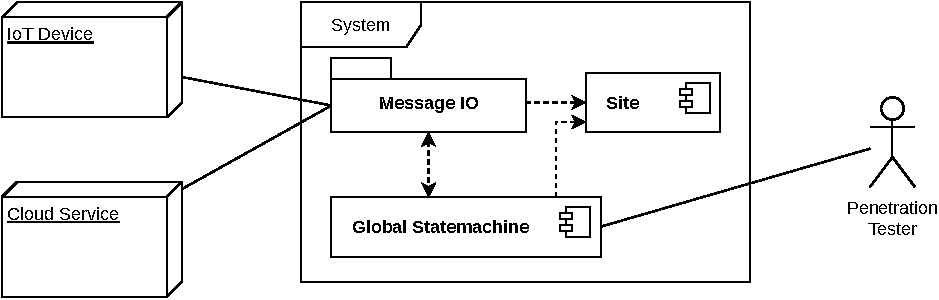
\includegraphics[width=12cm]{img/ch05/component-view-1.pdf}
    \captionof{figure}{High-level component diagram of the proxy application concept}
    \label{fig:component-view-1}
\end{figure}
As discussed in the previous chapter, the requirement \enquote{F2 Network Stacks} introduces the need for dynamically initialized objects which in this concept is implemented by making use of the factory pattern in the \enquote{Site}-component. This component allows for registering \emph{Factories} that are used to initialize objects. Similar to the implementation in the first prototype, factories initialize objects using metadata supplied from a configuration file.\\
Communication with other systems is encapsulated into the \enquote{Message IO}-package shown in figure \ref{fig:component-view-2}. Applications that are tested by penetration testers are connected to sockets provided by the \enquote{Gateway}-component and temporarily stored in a message queue to be processed by the network stacks organized by the \enquote{Global Statemachine}. Similar to the \enquote{Server}-interface used in the first prototype, gateways provide means of communicating with external systems and receiving and sending messages. They are highly abstract and meant to be used for implementing interfaces for any kind of communication protocols and technologies, such as \ac{IP}-based \ac{TCP} and \ac{UDP} communication but also other protocols such as USB, Bluetooth, ZigBee or KNX.
\begin{figure}[h]
    \centering
    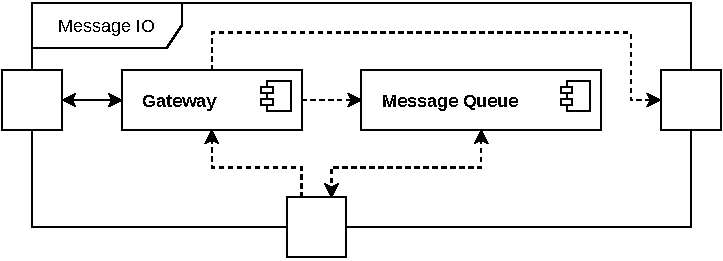
\includegraphics[width=12cm]{img/ch05/component-view-2-messageio.pdf}
    \captionof{figure}{The \enquote{Message IO}-package}
    \label{fig:component-view-2}
\end{figure}
It should be noted that the static view of the design is rather simple due to its dynamic runtime behaviour: many instances and relationships are only instantiated at runtime and not pre-determined.\\
Figure \ref{fig:app-activity-fsms} illustrates the recursive nature of this concept processing (dequeued) messages:
\begin{enumerate}
    \item A state-machine $F$ (initialized with the global state-machine instance) relays messages $M$ through its active state $S$'s network stack instance $N$.
    \item In $N$, all of its pipes $P$ process $M$ until the end of $N$ is reached ($P$ does not hold a reference to a succeeding pipe instance). If $F$ holds a reference to a succeeding \ac{FSM}, $F$ is set to this reference and the processes continues from step $1$.
    \item If $N$ does not hold a reference to a nested \ac{FSM}, the end of the network stack is reached and the direction of traversing the network stack is reversed.
    \item $P$ is set to $N$'s last pipe instance and $M$ is processed by $P$ until the start of $N$ is reached (i.e. $P$ does not hold a reference to a preceding pipe instance). If $F$ holds a reference to a preceding \ac{FSM} instance, $F$ is set to this reference, $N$ is set to $F$'s network stack reference and the process continues from step $4$.
    \item If $N$ does not hold a reference to a preceding \ac{FSM}, the beginning of the whole pipeline is reached and $F$ is the global state-machine.
\end{enumerate}


\section{Design \#1: Single Proxy Service}

\section{Design \#2: Distributed Proxy Services}

%\paragraph{Software Architecture} The system employs a server-client architecture that allows to

\emph{TBD} %TODO
\begin{itemize}
    \item \emph{Stream-based: treat communication as streams. message-based systems are simpler and supported by design}
    \item \emph{Server-client: proxy is server, client can interface to control + monitor, communication via REST + WS}
    \item \emph{State-machine: active network stack/pipeline dependent on state of the connection}
    \item \emph{NetStacks: series of pipelines, bound to states}
    \item \emph{Pipes: basic pipes, loose routing, injectable, specialized, generic processors + specialized encoders}
    \item \emph{Factory: parse state-machine and netstack configuration and instantiate + configure instances}
\end{itemize}